\documentclass[dvipdfmx]{jsarticle}
\usepackage[T1]{fontenc}
\usepackage[dvipdfmx]{hyperref}
\usepackage{lmodern}
\usepackage{latexsym}
\usepackage{amsfonts}
\usepackage{amssymb}
\usepackage{mathtools}
\usepackage{nccmath}
\usepackage{amsthm}
\usepackage{multirow}
\usepackage{graphicx}
\usepackage{wrapfig}
\usepackage{here}
\usepackage{float}
\usepackage{ascmac}
\usepackage{url}

\title{クラスタリング・分類・相関ルール分析に関する調査}
\author{文理学部情報科学科\\5419045 高林 秀}
\date{\today}

\begin{document}

\maketitle

\begin{abstract}
本稿は、今年度データ科学2のレポート課題として、「クラスタリング」、「分類(決定木)」および「相関ルール分析」の各分野に関して、各手法の特徴やアルゴリズムの説明、解説を行うものである。また、1年次に学習したlatexを使用したpdf作成の復習も兼ねるものである。
\end{abstract}

\section{目的}
本稿は、今年度データ科学2の最終レポート課題として「クラスタリング」、「分類(決定木)」および「相関ルール分析」の各分野に関して、各手法の特徴やアルゴリズムの説明、数式等の解説を行うものである。それぞれの分野の各手法の特徴やアルゴリズムに言及した上、使われている数式の解説を記載する。
\section{基礎導入}
\subsection{データマイニングとは}
まず、本稿で取り扱う分野の大元であるデータマイニングについて軽く説明する。データマイニングとはビックデータや企業の顧客情報など大量のデータが格納されたデータベースから機械学習や、統計計算等の手法でデータを分析し、そこから新たに有用な知識を発見しようという技術である。データマイニングでは、データから得られる情報を分析しそこから得ることのできる知識を取り出すことである。つまり、そこから先の得た知識をどう利用するかは人間の判断に委ねられている。すなわち、データマイニングで行うのは知識の発掘であり、発掘した知識が有用か、またどう活用するかは人間が判断する、ということだ。\par
大きく分けてデータマイニングは以下のように分類することができる。
\begin{enumerate}
  \item 仮説検証的データマイニング
  \begin{enumerate}
    \item 推定
    \item 分類
  \end{enumerate}
  \item 知識探索的データマイニング
  \begin{enumerate}
    \item 相関ルール分析(アソシエーションルール分析)
    \item クラスタリング
  \end{enumerate}
\end{enumerate}
上記の分類はあくまで大別であり、実際は手法により当てはまる分野は異なる。\par
仮説検証的データマイニングは、仮説に沿ってある課題を解決するためにデータ分析を行うことを示す。機械学習の手法のみならず従来までの統計的手法が使用されることも多い。\par
知識探索的データマイニングは、データベース上のデータから特定のルールや規則、パターンといった知識を探索するためにデータ分析を行うことを示す。こちらは機械学習やディープラーニング等の手法が多く用いられる。本稿で扱うのは、上記に示した「分類」、「クラスタリング」、「相関ルール分析」の3つである。
\subsection{機械学習について}
機械学習とは、コンピュータがある問題とその答えを使用して学習を行い、データに潜むパターン等を識別、発見する技術である。この機械学習は大きく3つに系統が別れている。初めに「教師あり学習」、次に「教師なし学習」、最後に「強化学習」である。そしてそこから更に、求める結果や手法によって「分類」「回帰」「クラスタリング」「次元削減」「Q-Learning」と細かく分割される。
\begin{figure}[H]
  \centering
  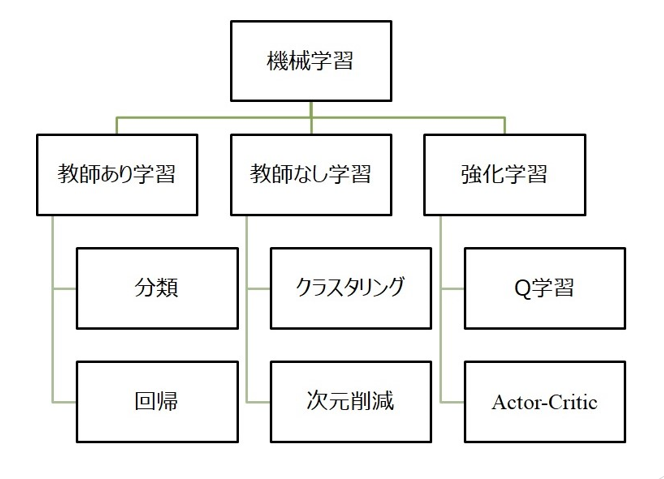
\includegraphics[scale=0.4]{images/ML.PNG}
  \caption{機械学習の枠組み}
\end{figure}
今回説明する、分類は上記分類の「教師あり学習」に、クラスタリングは「教師なし学習」に該当する。教師あり学習と教師なし学習についての具体的な説明は本稿では省略するが、以下にその件に関して記載したレポートのURLを添付する。
\begin{itemize}
  \item 機械学習に関する説明をした過去のレポート:\url{https://drive.google.com/file/d/1wyoRO20UmgiYsxAjkFKLzxhwPvv-xhbx/view?usp=sharing}
\end{itemize}
\section{クラスタリング}
クラスタリングとは、データのグループ分けを行うことをいい、クラスタリングの結果で生じた各データ集合をクラスタと呼ぶ。このクラスタには同じ様な性質をもったデータが集められている。前章で示したとおりクラスタリングは与えられたデータから計算によって自動的にデータの分類、グルーピングを行うので、機械学習では教師なし学習に分類される。\par
クラスタリングは、知識探索的な手法であるので得られた結果は何らかの基準にしたがってクラスタが形成されている。よって、客観的な証拠としてクラスタリングを用いるのは適切ではなく、データの要約など知識や知見を得るために使用するのが適切である。\par
なお、今後の説明で登場するクラスタ内距離やクラスタ間距離などの用語については、今回の課題の説明範囲外なので以下のレポートを参照いただきたい。
\begin{itemize}
  \item クラスタリングの基本に関する説明レポート:\url{https://drive.google.com/file/d/1JP3DnVNmH3kOtEULt73u79zJTb1B1Wvq/view?usp=sharing}
\end{itemize}
クラスタリングは以下に示すように、階層的クラスタリングと非階層的クラスタリングの2つに大別される。
\begin{enumerate}
  \item 非階層的クラスタリング
  \begin{enumerate}
    \item k-平均法(k-means)
  \end{enumerate}
  \item 階層的クラスタリング
  \begin{enumerate}
    \item 凝集型(階層的併合型)
    \item 分岐型
  \end{enumerate}
\end{enumerate}
その他にも、クラスタ間の密度に基づく手法や、格子に基づく手法などに分けることもできるが本稿では省略する。
\subsection{非階層的クラスタリング}
非階層的クラスタリングは、予め分割するクラスタ数$K$を定めたとき、クラスタ内距離を最小にしつつかつクラスタ間距離を最大にするようにクラスタを決定する方法である。このクラスタ数$K$は人間が定めるハイパラメータであり、この$K$の値によってクラスタリング結果は大きく変化する可能性がある。このクラスタ数$K$を自動的に決定する手法はいくつか考案されているが、本稿での説明は省略する。\par
以下は、非階層的クラスタリングの流れの概要である。
\begin{enumerate}
  \item クラスタ数$K$を定める。
  \item データを$k$分割する。
  \item なにかの基準や手法を用いてデータ分割が改善するように、データ分割を繰り返す。
  \item 3の結果、改善される度合いが小さくなればクラスタリング終了。
\end{enumerate}
非階層的クラスタリングの長所として、計算量の少なさが挙げられるだろう。これは後述する手法からも分かるとおり、予め分割するクラスタ数$K$にしたがってデータを分けていく。したがって、階層的クラスタリングよりも計算量が小さくなるという利点がある。よって、データ量が大きい場合(例:ビックデータ分析)のデータ分析に適した手法とされている。\par
反対に、短所として「初期値依存性」が挙げられるだろう。これは、クラスタリングを行う際、最初に$K$個の初期中心点を選択する必要があり、この初期中心点の選択によってクラスタリング結果が大きく変化するという問題である。
\begin{figure}[H]
  \centering
  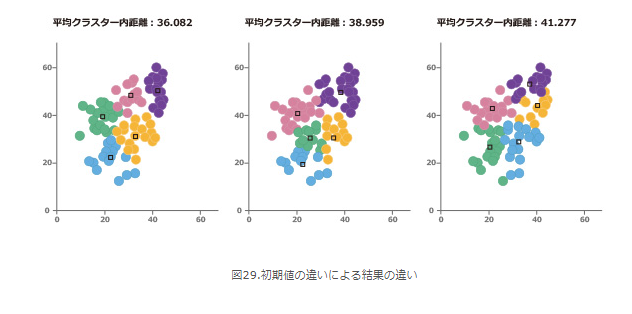
\includegraphics[scale=0.4]{images/k-problem.png}
  \caption{非階層的クラスタリングの初期値依存性の例}
  出典:\url{https://www.albert2005.co.jp/knowledge/data_mining/cluster/non-hierarchical_clustering}
\end{figure}
よって、非階層的クラスタリングを行う際には何回かクラスタリングを実行し、平均クラスタ内距離が最小となる初期中心点を選択する必要が生じる。\par
次は非階層的クラスタリングの代表的手法であるk-平均法(k-means)について説明する。
\subsubsection{k-平均法(k-means)}
k-平均法では以下の目的関数を利用する。この目的関数を最小化するようにデータの分割を行いクラスタを形成していく手法である。
\begin{gather*}
  \Sigma_{k=1}^{K}\Sigma_{x_{i}\in C_{k}}(x_{i}-c_{k})^{2}
\end{gather*}
k-平均法のアルゴリズムは以下に示すとおりである。
\begin{enumerate}
  \item クラスタ数$K$定める。
  \item ある手法に基づいてデータ集合を$K$個のクラスタに分割し、その結果を$C_{n}$とする
  \item 2の結果を$C_{pre}$として保持しておく\par
  以降は、$C_{n}$と$C_{pre}$が一致するまで繰り返しをする。
  \item 各クラスタの重心を計算し、それを新たなクラスタの中心点とする
  \item 各データと中心点との距離を計算し、最も近い中心点のクラスタへの割当を行う→この結果を$C_{n}$とする:目的関数の値が最小化するようにクラスタを更新する
  \item $C_{n}$と$C_{pre}$が一致した場合はクラスタリングを終了し、そうでない場合はもう一度3を行う。\par
  クラスタリング終了時
  \item $C_{n}$を結果として出力する
\end{enumerate}
k-平均法では、各クラスタの重心とクラスタ内距離の総和の局所最適解\footnote{ある範囲における関数の最小値(極小値)のこと。その関数の真の最小値(極小値)は大域的最適解と呼ばれる。}を求めていく。この局所最適解が収束するまで、クラスタ割当の更新と重心の再計算を行う。\par
なお初期クラスタの形成に関しては次の3通りの手法が挙げられる。
\begin{itemize}
  \item 各データに対して、ランダムに1から$K$個のいずれかのクラスタに割当を行う方法
  \item データ全体からランダムに$K$個のデータを選択し、それぞれ{s1~sK}とする。{s1~sK}以外の各データは、{s1~sK}の中で最も近いsi(s1~sKのうちから1つ)のクラスタに割り当てる方法。
  \item データのある空間からランダムに$K$個の点を生成し選択する。それぞれ{s1~sK}とする。各データは{s1~sK}の中で最も近いsi(s1~sKのうちから1つ)のクラスタに割り当てる方法。
\end{itemize}

\subsection{階層的クラスタリング}
前章の非階層的クラスタリングとは異なり、階層的クラスタリングでは予めクラスタ数$K$を定める必要はない。階層的クラスタリングでは、似た性質を持つデータ同士を1つずつグルーピングしていくようにクラスタを形成する。データを1つ1つ比較ししていき、似ているデータ同士、およびクラスタを新たなクラスタとして併合する。そうすると、最終的に階層構造のようなクラスタが出来上がるので、階層的クラスタリングと呼ばれている。\par
先に示したが、階層的クラスタリングには凝集型と分岐型に大別することができる。
\paragraph{凝集型}
凝集型は階層併合的クラスタリングとも呼ばれ、各データを1つのクラスタとして考え各クラスタをボトムアップに併合することで、新たなクラスタを形成する手法である。手順の概要は下記に示すとおり。
\begin{enumerate}
  \item 各データをそれぞれ1つのクラスタと見なす
  \item クラスタの数が1つになるまで次の操作を繰り返す
  \begin{enumerate}
    \item それぞれクラスタ間で距離を算出する
    \item 最も距離が小さいペア同士を新たなクラスタとして併合する
  \end{enumerate}
\end{enumerate}
図で示すと以下のようになる。左から順番に進行する。
\begin{figure}[H]
 \begin{minipage}{0.5\hsize}
  \begin{center}
   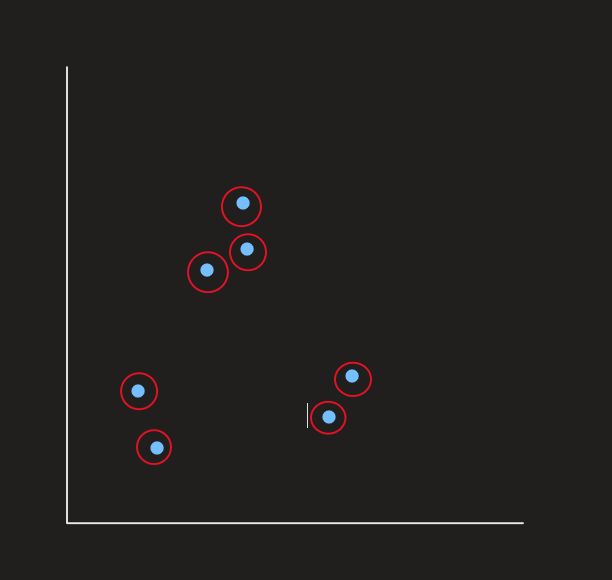
\includegraphics[scale=0.3]{images/gyousyu01.png}
  \end{center}
  \caption{1.各データをそれぞれ1つのクラスタと見なす}
  \label{fig:one}
 \end{minipage}
 \begin{minipage}{0.3\hsize}
  \begin{center}
   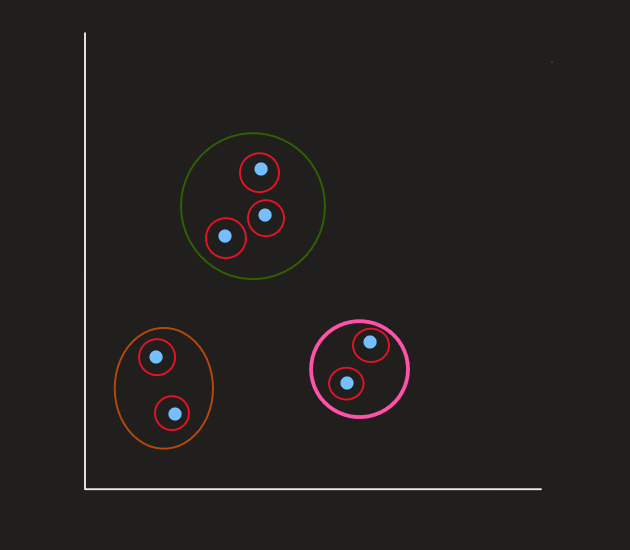
\includegraphics[scale=0.3]{images/gyousyu02.png}
  \end{center}
  \caption{2~(a),(b)クラスタの併合}
  \label{fig:two}
 \end{minipage}
 \begin{minipage}{0.5\hsize}
  \begin{center}
   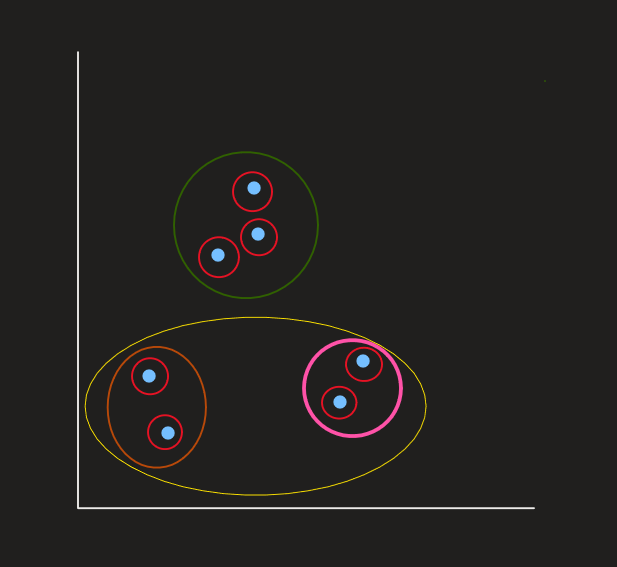
\includegraphics[scale=0.3]{images/gyousyu03.png}
  \end{center}
  \caption{3.クラスタの併合その2}
  \label{fig:two}
 \end{minipage}
 \begin{minipage}{0.5\hsize}
  \begin{center}
   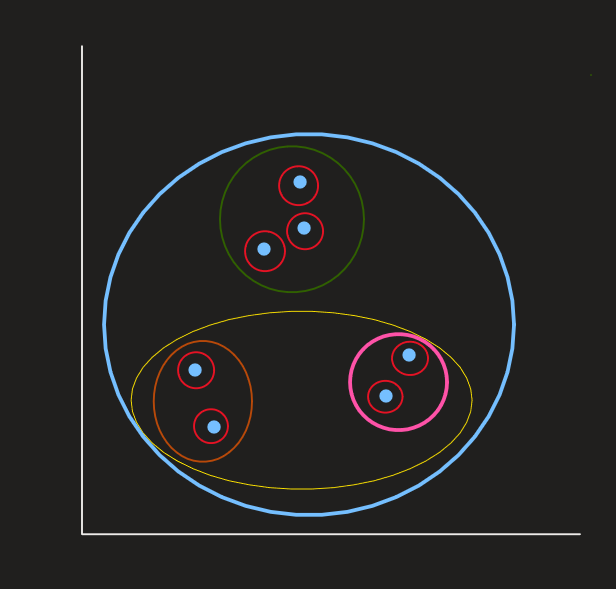
\includegraphics[scale=0.3]{images/gyousyu04.png}
  \end{center}
  \caption{4.クラスタ数が1になったのでクラスタリング終了}
  \label{fig:two}
 \end{minipage}
\end{figure}
より形式的に示す以下の様なアルゴリズムが出来上がる。
\begin{verbatim}
  X:クラスラリング対象のデータ集合
  C := {{x} | x ∈ X}:クラスタの集合C
  while |C| > 1 {
    <C_a, C_b>:=argmin_C_i,C_j ∈ C(D(C_i, C_j))
    C := (C\{C_a, C_b})∪{C_a∪C_b}
  }
\end{verbatim}
凝集型クラスタリングの具体的な計算手法には、利用するクラスタ間距離に応じて下記のものが存在する。
\begin{itemize}
  \item ウォード法(ward法)
  \item 群平均法
  \item 重心法
  \item 最短距離法(単リンク法,単連結法)
  \item 最長距離法(完全リンク法,完全連結法)
  \item 群間平均法
\end{itemize}
\begin{itemize}
  \item $C_{x}$:クラスタの集合
  \item $D(C_{x}, C_{y})$:クラスタ間距離
  \item $M(C_{x})$:クラスタの重心
\end{itemize}
\paragraph{最短距離法}
最短距離法は、異なるクラスタに属している2データ間距離の最小値をクラスタ間距離とする手法である。すなわち、最近点距離である。
\begin{center}
\begin{eqnarray*}
    D(C_{g}, C_{h}) = min_{i \in C_{g}, j \in C_{h}}(dist(i, j)
\end{eqnarray*}
\end{center}
\paragraph{最長距離法}
最長距離法は、異なるクラスタに属している2データ間距離の最大値をクラスタ間距離とする手法である。すなわち、最遠点距離である。
\begin{center}
  \begin{eqnarray*}
    D(C_{g}, C_{h}) = max_{i \in C_{g}, j \in C_{h}}(dist(i, j))
  \end{eqnarray*}
\end{center}
\paragraph{群間平均法}
群間平均法は、異なるクラスタに属している2データ間距離の平均値をクラスタ間距離とする手法である。すなわち、平均距離である。
\begin{center}
  \begin{eqnarray*}
    D(C_{g}, C_{h}) = \frac{1}{|C_{g}|\times |C_{h}|}\Sigma_{i \in C_{g}, j \in C_{h}}dist(i,j)
  \end{eqnarray*}
\end{center}
\paragraph{重心法}
重心法は、各クラスタの重心を求め、その距離をクラスタ間距離とする手法である。すなわち、重心間距離である。
\begin{center}
  \begin{eqnarray*}
    D(C_{g}, C_{h}) = dist(M(C_{g}), M(C_{h}))
  \end{eqnarray*}
\end{center}
\paragraph{ウォード法}
ウォード法は「重心との誤差の改善度合い」に着目し計算する手法である。
\begin{center}
\begin{eqnarray*}
  D(C_{g}, C_{h}) = E(C_{g}\cup C_{h}) - E(C_{g}) - E(C_{h})
  = E(C_{g}\cup C_{h}) - (E(C_{g}) + E(C_{h})) \\
  なお、
  E(C) = \Sigma_{x\in C}dist(x, M(C))^{2} : 重心からの距離の二乗和\\
  ※D(C_{g}, C_{h}):クラスタまたはデータの「併合後の誤差」-「併合前の誤差」
\end{eqnarray*}
\end{center}
\paragraph{分岐型}
凝集型とは異なりトップダウンに各データを分割することでクラスタを形成する。データ集合全体を1つのクラスタと見なし、徐々に小さいクラスタへ分割していく手法である。現在のところあまり使用されていない手法と言える。\par
なお、本稿では分岐型の具体的な説明は省略するが、具体的手法の例として「Diana法」が存在する。\par
\subsection{非階層的クラスタリングと階層的クラスタリングの長所と短所}
前章でも述べたが、非階層的クラスタリングの長所として、計算量の少なさが挙げられるだろう。反対に、短所として「初期値依存性」が挙げられるだろう。\par
階層的クラスタリングの長所として、前章の計算手法で紹介したとおり重心を用いない手法であれば様々な類似度を利用することができる点が挙げられる。加えて、クラスタを併合する際の順番が分かりやすいので、細かくクラスタの変化の様子を追うことができる。これは、階層的クラスタリングの結果として使用する「デンドログラム」の存在が大きな要因になっている。後述する決定木のように、クラスタ併合の課程が樹形図で可視化することができるので、非階層的クラスタリングよりも結果の説明がしやすい。
反対に、欠点としてデータ数が多いと樹形図の把握が困難になり、理解困難になる。また、各事例間に類似度の差が小さい場合、樹形図の鎖状化の発生により、全体的なクラスタを把握するのが難しくなる点がある。その他にも、使用する手法によって様々な問題点を抱えている。以下その一例を示す。
\begin{itemize}
  \item 郡平均法を使用した場合:デンドログラムの反転現象が起こる可能性がある。これはクラスタ間距離の現象により、デンドログラムが交差してしまう現象である。
  \begin{figure}[H]
    \centering
    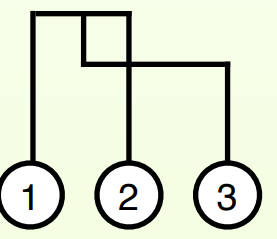
\includegraphics[scale=0.4]{images/dendoroHanten.png}
    \caption{デンドログラムの反転現象の例}
    出典:\url{https://www.kamishima.net/archive/clustering.pdf}
  \end{figure}
  \item 最短距離法:空間濃縮の発生$\Rightarrow$併合後の新クラスタは次の併合の対象となる可能性が加速度的に増加する。
  \item 最長距離法:空間拡張$Rightarrow$併合後の新クラスタは次の併合の対象となる可能性が加速度的に減少する。
\end{itemize}
\section{分類:決定木構築TDIDT}
分類は先に示したとおり、機械学習の教師あり学習に区分される。分類学習では、事前に定められたカテゴリ、およびクラスに入力データを分類することを行う。その一手法として決定木というものが存在する。\par
\subsection{決定木について}
決定木は「木構造を利用した機械学習手法」である。分類を行う決定木を「分類木」、回帰(連続値の予測)を行う決定木は「回帰木」と呼ばれる。決定木では任意の属性の属性値による条件分岐によって、データを徐々に分割することで結果を出力する。したがって、生成される木構造の枝は分割の結果ラベルを、葉は予測、分類されるクラスの結果を、各ノードは属性に関する分割テスト含んでいる。\par
決定木を使用する例として、ミカンとリンゴを分類する場合を考える。下記の図のように、ミカンの画像を4枚、リンゴの画像を2枚の計6枚の画像データセットがあるとする。
これを、ある条件Aを定め、それに当てはまるもの、そうでないものを分割する。この操作を分割テストという。分割テストの結果によって次の分割テスト行うか否かが決定され、最終的に、ミカンとリンゴが図のように分類される。これが決定木の大まかな流れである。
\begin{figure}[H]
  \centering
  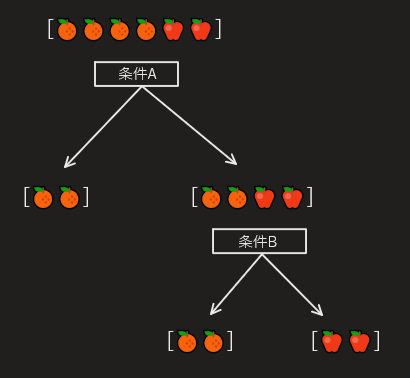
\includegraphics[scale=0.6]{images/decition_ex1.PNG}
  \caption{ミカンとリンゴの分類木}
\end{figure}
以下簡単に決定木の長所、短所をまとめる。
\begin{table}[H]
  \begin{center}
    \caption{決定木のメリット・デメリット}
    \begin{tabular}{|c|c|} \hline
      メリット & デメリット \\ \hline
      ・学習結果の可読性が高く結果の根拠を説明しやすい & ・条件分岐が複雑になるほど過学習しやすい\\
      ・データの前処理が少なく済むことが多い & ・精度が突出して良いわけではない\\
      ・予測時に必要な計算量が小さい & \\
      ・回帰、分類の両方に対応可能 & \\ \hline
    \end{tabular}
    \label{hyo01}
  \end{center}
\end{table}
\subsection{TDIDTについて}
決定木構築手法の代表例として、TDIDT法(Top Down Induction of Decision Trees)がある。この手法は、比較的簡単にコンパクトかつ正確な決定木を作ろうとする概念、すなわちヒューリスティックスに基づいた決定木構築法である。ここでいうTop Downとは、木の根から作るという意味で、Inductionとは、帰納推論、すなわちデータからモデルを構築するという意味である。\par
TDIDTの大まかな流れは次の通り。
\begin{enumerate}
  \item 根となるデータ集合を用意する。
  \item ある基準(情報利得・情報利得比・ジニ係数)で属性を選ぶ。
  \item 選ばれた属性の属性値ごとにデータを分割する。
  \item 各枝に対して、3を繰り返す。
  \item 停止条件を満たす場合、その枝の分割を終了とする。
\end{enumerate}
分割属性の選択は、できるだけその属性で分割したときにクラス分布が偏れば、しっかりとデータを分類できるので良い分割基準となる。\par
このとき、分割属性の選択基準として考えられる情報利得・情報利得比・ジニ係数について説明する。なお、本稿では自己情報量等の基本的な数式の説明は省略する。この部分に関しては、以下のリンクから決定木構築のレポートを参照いただきたい。
\begin{itemize}
  \item 決定木構築のレポート:\url{https://drive.google.com/file/d/1QviNpUqGr6yGqpJYqp1gyfWtksf35V6o/view?usp=sharing}
\end{itemize}
\subsubsection{情報利得}
情報利得とは一言で言えば「クラスの偏りがどの程度進んだか」を表す数値である。データセット$D$のおける属性$A$の情報利得の計算式は下記。
\begin{center}
  \begin{align*}
    Gain_{A}(D) = H(D) - H_{A}(D) \\
  \end{align*}
\end{center}
この値が大きいほど、分割テストに適した良い属性ということになる。
$D$を分割する前のエントロピーが$H(D)$で、属性$A$での分割後のエントロピーが$H_{A}(D)$であり、それぞれ下記式で示すことができる。
\begin{center}
  $I(c, D)|c:クラス, D:データセット(データ集合)$とすると、
  \begin{center}
    \begin{align*}
      I(c, D) = -\log_2 P_{D}(c) \\
    \end{align*}
    ※$P_{D}(c)$:$D$中のデータのクラスが$c$となる確率
  \end{center}
  \begin{align*}
    H(D)=\Sigma_{c \in C}P_{D}(c) \times I(c, D)=-\Sigma_{c \in C}P_{D}(c)\log_2 P_{D}(c) \\
  \end{align*}
  \begin{align*}
    H_{A}(D)=\Sigma_{a \in A}p_{D}(a) \times H(D_{a}) \\
  \end{align*}
  $P_{D}(a)$:$D$中のデータの属性$A$の属性値が$a$となる確率。
\end{center}
すなわち、クラス分布を偏らせるためには、情報利得が大きい属性を選択すれば良い。すなわち\textbf{情報利得 = 分割前のエントロピー - 分割後の各エントロピーの重み付き平均}ということになる。\par
しかし、情報利得にはある問題点がある。それは、分割数の大きい属性に対して優先的に高い数値を与えてしまうという点だ。これは、例えば各事例に振られるID番号の例を考えれば分かりやすい。ID番号は事例ごとに1つの数値を割り振っている。したがって、どの属性よりもデータの分割数が大きい属性ということになる。このID属性を分割テストに用いた場合、ある意味完全にデータを分類できるが、ID番号はただの番号、データの順番なので意味をなさない。この様な欠点を補うため、情報利得比と呼ばれる分割基準がある。
\subsubsection{情報利得比}
情報利得比とは、情報利得を分割情報量で正規化した数値である。
\paragraph{分割情報量}分割数が大きい属性に対して、より大きな値をとる性質を持つ。
\begin{center}
  \begin{align*}
    SI_{A}(D) = \Sigma_{a\in A}P_{D}(a) \times I(a, D) = \Sigma_{a\in A}P_{D}(a)\log_2 P_{D}(a)
  \end{align*}
\end{center}
情報利得比$GainRaito_{A}(D)$は下記式で計算される。
\begin{center}
  \begin{align*}
    GainRaito_{A}(D) = \frac{Gain_{A}(D)}{SI_{A}(D)}
  \end{align*}
\end{center}
\subsubsection{ジニ係数}







\section{相関ルール分析}
\end{document}
